\documentclass[12pt,a4paper]{article}

\usepackage[T1]{fontenc}
\usepackage[utf8]{inputenc}
\usepackage{lmodern}
\usepackage{amsmath,amssymb}
\usepackage{graphicx}
\usepackage{geometry}
\usepackage{enumitem}
\usepackage{fancyhdr}
\usepackage{float}

\geometry{
	top=2.0cm,
	bottom=2.0cm,
	left=2.2cm,
	right=2.2cm,
	headheight=15pt
}

\setlength{\parindent}{0pt}
\setlength{\parskip}{0pt}
\setlist[enumerate,1]{label=(\roman*),leftmargin=1.1cm,itemsep=0.65em,topsep=0.5em}

\pagestyle{fancy}
\fancyhf{}
\fancyhead[L]{\small Laboratório de Controle Aplicado}
\fancyhead[R]{\small Lista de Fixação 1}
\fancyfoot[L]{\footnotesize Prof. Dr. Sergio Ronaldo B. Santos\\Prof. Dr. André Marcorin de Oliveira}
\fancyfoot[R]{\footnotesize Page \thepage}
\renewcommand{\headrulewidth}{0.4pt}
\renewcommand{\footrulewidth}{0pt}

\fancypagestyle{firstpage}{
	\fancyhf{}
	\fancyfoot[C]{\thepage}
	\renewcommand{\headrulewidth}{0pt}
	\renewcommand{\footrulewidth}{0pt}
}

\begin{document}
	\thispagestyle{firstpage}
	
	\begin{minipage}[c]{0.48\textwidth}
		
\includegraphics[width=3.5cm]{images/logo-000.png}
	\end{minipage}%
	\begin{minipage}[c]{0.52\textwidth}
		\raggedleft
		
\includegraphics[width=2.4cm]{images/logo-001.png}
	\end{minipage}
	
	\vspace{0.9cm}
	
	\begin{center}
		{\LARGE Laboratório de Controle de Sistemas Dinâmicos\par}
		\vspace{0.7cm}
		{\LARGE Laboratório 1\par}
		\vspace{0.9cm}
		{\large Prof. Dr. Sergio Ronaldo B. Santos\par}
		{\large Aluno: Leonardo Tomasela Leal\par}
		{\large RA: 170291\par}
		\vspace{0.25cm}
		% {\large Prof. Dr. André Marcorin de Oliveira\par}
		%\vspace{0.6cm}
		%{\large Segundo Semestre de 2022\par}
		
		\vspace{1.0cm}
		{\LARGE Exercícios\par}
	\end{center}
	
	\vspace{0.5cm}
	
	\textbf{1.)} Considere as seguintes equações diferenciais:
	
	\begin{equation}
		\dot{x}+ax=au
		\label{eq:primeira-ordem}
	\end{equation}
	
	e
	
	\begin{equation}
		\ddot{x}+\beta\gamma\dot{x}+\gamma^{2}x=\gamma^{2}u
		\label{eq:segunda-ordem}
	\end{equation}
	
	\begin{enumerate}
		\item Qual a ordem da equação diferencial da Equação~\eqref{eq:primeira-ordem}? E da Equação~\eqref{eq:segunda-ordem}?
		
		\textbf{Resposta:} A equação~\eqref{eq:primeira-ordem} é de primeira ordem e a equação~\eqref{eq:segunda-ordem} é de segunda ordem.
		
		\item Implemente \eqref{eq:primeira-ordem} para $u=1$ no Simulink. Escolha valores arbitrário para $a$. Qual o comportamento de $x$?
		
		\textbf{Resposta:}
		
		Sistema implementado:
		\begin{figure}[H]
			\centering
			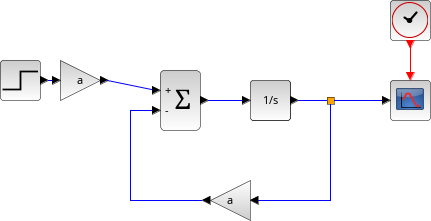
\includegraphics[width=0.75\textwidth]{images/sistema1_ii.png}
		\end{figure}
		\begin{enumerate}
			\item $a = 1:$
			\begin{figure}[H]
				\centering
				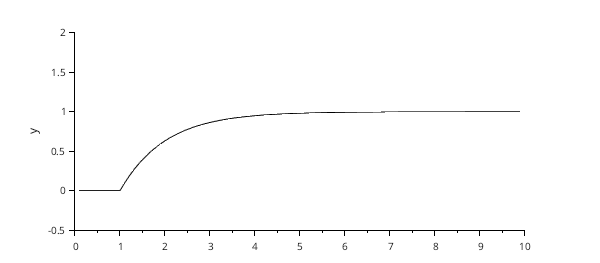
\includegraphics[width=0.75\textwidth]{images/a_1.png}
			\end{figure}
			\item $a = 5:$
			\begin{figure}[H]
				\centering
				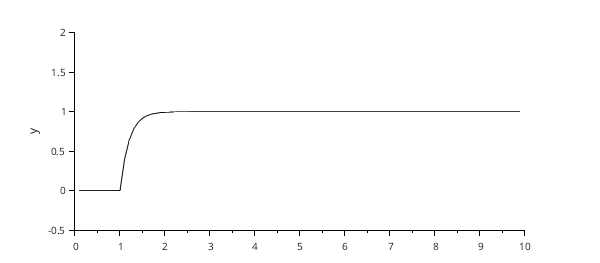
\includegraphics[width=0.75\textwidth]{images/a_5.png}
			\end{figure}
			\item $a = 10:$
			\begin{figure}[H]
				\centering
				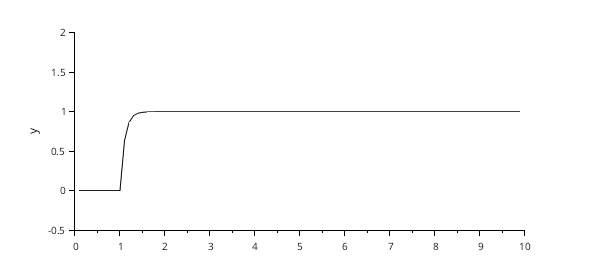
\includegraphics[width=0.75\textwidth]{images/a_10.png}
			\end{figure}
		\end{enumerate}
		
		Pode-se perceber que, quando maior o valor de $a$, maior a velocidade de resposta do sistema.
		
		
		\newpage
		
		\item Implemente \eqref{eq:segunda-ordem} para $u=1$ no Simulink. Escolha valores arbitrário para $\beta$ e $\gamma$. Qual o comportamento da saída $x$? Se fixarmos $\beta$, o que acontece se aumentamos o valor de $\gamma$? E vice-versa?
		
		\textbf{Resposta:}
		
		Sistema implementado:
		\begin{figure}[H]
			\centering
			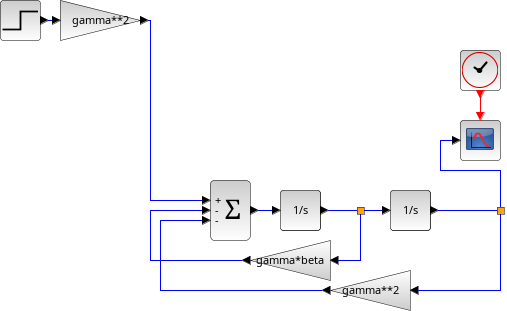
\includegraphics[width=0.75\textwidth]{images/sistema1_iii.png}
		\end{figure}
		
		\begin{enumerate}
			\item $\gamma = 1;\ \beta = 1:$
			\begin{figure}[H]
				\centering
				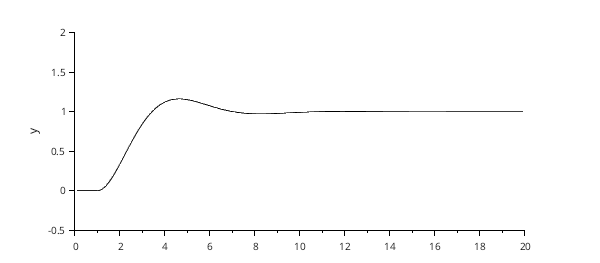
\includegraphics[width=0.75\textwidth]{images/beta_gamma_1.png}
			\end{figure}
			\item $\gamma = 5;\ \beta = 1:$
			\begin{figure}[H]
				\centering
				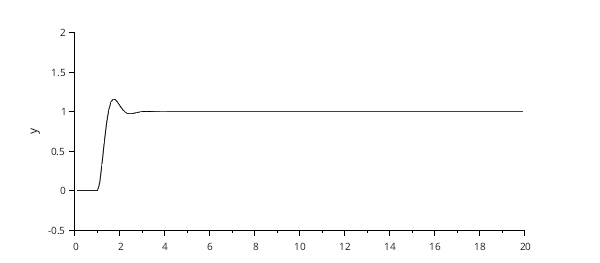
\includegraphics[width=0.75\textwidth]{images/gamma_5.png}
			\end{figure}
			\newpage
			\item $\gamma = 10;\ \beta = 1:$
			\begin{figure}[H]
				\centering
				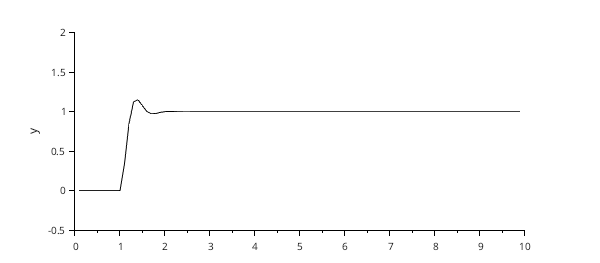
\includegraphics[width=0.75\textwidth]{images/gamma_10.png}
			\end{figure}
			\item $\gamma = 1;\ \beta = 5:$
			\begin{figure}[H]
				\centering
				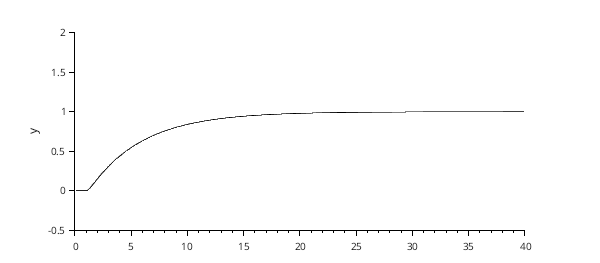
\includegraphics[width=0.75\textwidth]{images/beta_5.png}
			\end{figure}
			\item $\gamma = 1;\ \beta = 10:$
			\begin{figure}[H]
				\centering
				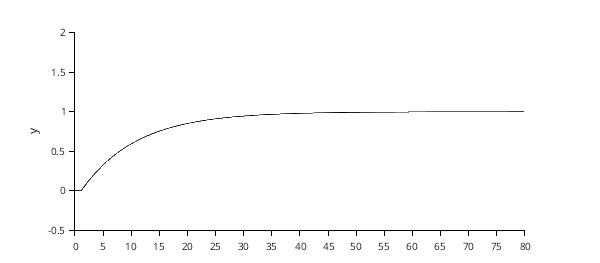
\includegraphics[width=0.75\textwidth]{images/beta_10.png}
			\end{figure}
		\end{enumerate}
		
		Pode-se observar que, quando $\gamma$ é aumentado, há um aumento na velocidade de resposta do sistema. Quando $\beta$ é aumentado, há um aumento no amortecimento do sistema.
		
		\newpage
		
		\item Em posse dos comportamentos levantados anteriormente, quais as diferenças qualitativas entre \eqref{eq:primeira-ordem} e \eqref{eq:segunda-ordem}? Quais sistemas físicos poderiam ser representados por \eqref{eq:primeira-ordem} e \eqref{eq:segunda-ordem}?
		
		\textbf{Resposta:}
		
		A equação \eqref{eq:primeira-ordem} é um sistema de primeira ordem, apresentando uma resposta exponencial sem oscilações. Pode representar, por exemplo, um circuito RC. Já a equação \eqref{eq:segunda-ordem} é um sistema de segunda ordem, cujo comportamento depende dos parâmetros \(\beta\) e \(\gamma\), podendo ser subamortecido, criticamente amortecido ou superamortecido. Pode representar, por exemplo, um circuito RLC ou um sistema massa-mola-amortecedor.
	\end{enumerate}
	
	\textbf{2.)} Considere as seguintes funções de transferência:
	
	\[
	G_{1}(s)=\frac{\alpha}{s+\alpha}
	\]
	
	e
	
	\[
	G_{2}(s)=\frac{\omega_n^{2}}{s^{2}+2\xi\omega_n s+\omega_n^{2}}
	\]
	
	\begin{enumerate}
		\item Qual a ordem do sistema descrito por $G_{1}(s)$? E por $G_{2}(s)$?
		
		\textbf{Resposta:}
		
		O sistema descrito por $G_1(s)$ é de primeira ordem; O sistema descrito por $G_2(s)$ é de segunda ordem
		
		\item Escolha valores arbitrário para $\alpha$ em $G_{1}(s)$ e aplique um degrau ao sistema no Simulink. Qual o comportamento da saída? O que acontece se aumentamos o valor de $\alpha$?
		
		\textbf{Resposta:}
		
		Sistema implementado:
		
		\begin{figure}[H]
			\centering
			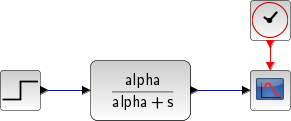
\includegraphics[width=0.75\textwidth]{images/sistema2_ii.png}
		\end{figure}
		
		\newpage
		\begin{enumerate}
			\item $\alpha = 1:$
			\begin{figure}[H]
				\centering
				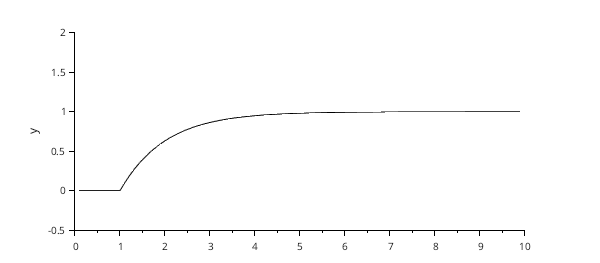
\includegraphics[width=0.75\textwidth]{images/alpha_1.png}
			\end{figure}

			\item $\alpha = 5:$
			\begin{figure}[H]
				\centering
				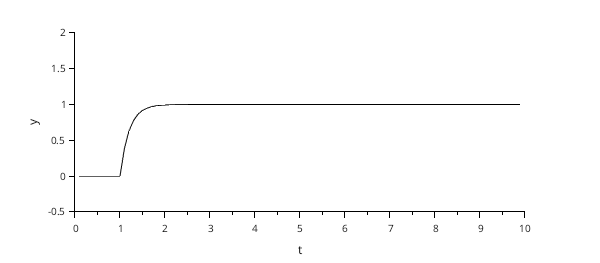
\includegraphics[width=0.75\textwidth]{images/alpha_5.png}
			\end{figure}
			\item $\alpha = 10:$
			\begin{figure}[H]
				\centering
				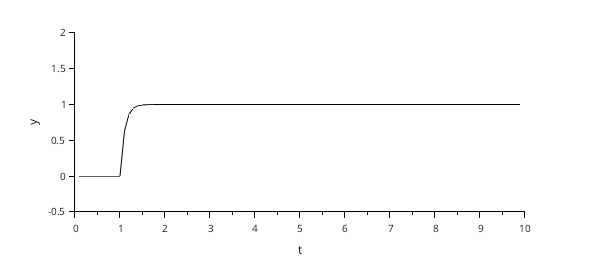
\includegraphics[width=0.75\textwidth]{images/alpha_10.png}
			\end{figure}
		\end{enumerate}
		
		Pode-se observar que a saída é uma resposta exponencial, partindo do valor inicial e tendendo ao valor do degrau aplicado. Conforme o valor de $\alpha$ aumenta, a velocidade de resposta do sistema aumenta.
		
		\newpage
		
		\item Escolha valores arbitrário para $\omega_n$ e $\xi$ em $G_{2}(s)$ e aplique um degrau ao sistema no Simulink. Qual o comportamento da saída? Se fixarmos $\omega_n$, o que acontece se aumentamos o valor de $\xi$? E vice-versa?
		
		\textbf{Resposta:}
		
		Sistema implementado:
		
		\begin{figure}[H]
			\centering
			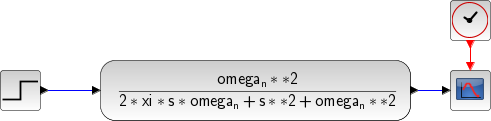
\includegraphics[width=0.75\textwidth]{images/sistema2_iii.png}
		\end{figure}
		
		
		\begin{enumerate}
			\item $\omega = 1;\ \xi = 1:$
			\begin{figure}[H]
				\centering
				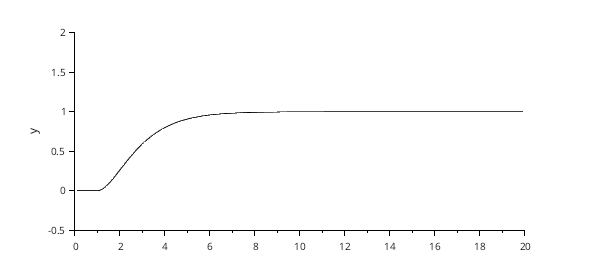
\includegraphics[width=0.75\textwidth]{images/omega_xi_1.png}
			\end{figure}
			\item $\omega = 5;\ \xi = 1:$
			\begin{figure}[H]
				\centering
				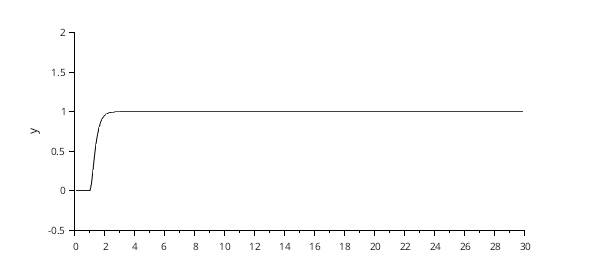
\includegraphics[width=0.75\textwidth]{images/omega_n_5.png}
			\end{figure}
			
			\newpage
			\item $\omega = 10;\ \xi = 1:$
			\begin{figure}[H]
				\centering
				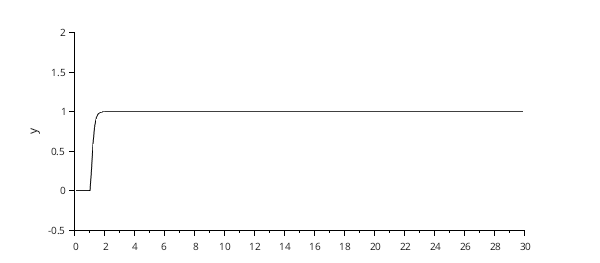
\includegraphics[width=0.75\textwidth]{images/omega_n_10.png}
			\end{figure}
			\item $\omega = 1;\ \xi = 5:$
			\begin{figure}[H]
				\centering
				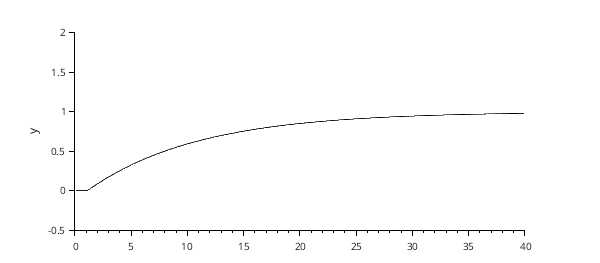
\includegraphics[width=0.75\textwidth]{images/xi_5.png}
			\end{figure}
			\item $\omega = 1;\ \xi = 10:$
			\begin{figure}[H]
				\centering
				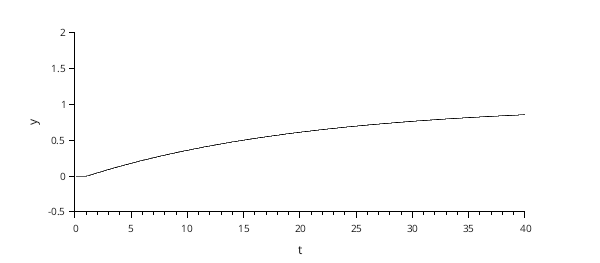
\includegraphics[width=0.75\textwidth]{images/xi_10.png}
			\end{figure}
		\end{enumerate}
		
		Pode-se observar que conforme valor de $\omega_n$ aumenta, a velocidade de resposta do sistema aumenta, conforme o valor de $\xi$ aumenta, aumenta-se o amortecimento do sistema.
		
		\newpage
		
		\item Em posse dos comportamentos levantados anteriormente, quais as diferenças qualitativas entre $G_{1}(s)$ e $G_{2}(s)$? Quais sistemas físicos poderiam ser representados por $G_{1}(s)$ e $G_{2}(s)$?
		
		\textbf{Resposta:}
		
		O sistema descrito por $G_1(s)$ é um sistema de primeira ordem, apresentando uma resposta exponencial sem oscilações. Pode representar, por exemplo, um circuito RC. Já o sistema descrito por $G_2(s)$ é um sistema de segunda ordem, cujo comportamento depende dos parâmetros \(\omega_n\) e \(\xi\), podendo ser subamortecido, criticamente amortecido ou superamortecido. Pode representar, por exemplo, um circuito RLC ou um sistema massa-mola-amortecedor.

	\end{enumerate}
	
\end{document}
